\documentclass{article}

\usepackage{pdfpages}
\usepackage{siunitx}
\usepackage[utf8]{inputenc}
\usepackage[toc,page]{appendix}
\usepackage{amsmath,mathrsfs}
\usepackage{lmodern}
\usepackage{fullpage}
\usepackage{units}
\usepackage{float}
\usepackage{icomma}
\usepackage{color}
\usepackage{graphicx}
\usepackage{ gensymb }
\usepackage{bbm}
\usepackage{verbatim}
\usepackage[T1]{fontenc}
\usepackage{caption}
\usepackage{tikz}
\usepackage{amssymb}
\usepackage{hyperref}
\usepackage{graphicx}
\usepackage{braket}
\usepackage{wrapfig}
\usepackage[a4paper, total={6in, 9in}]{geometry}
%\usepackage[parfill]{parskip}
%\usepackage[table]{xcolor}
%\usepackage[margin=1in]{geometry}
\usepackage{tabularx}
\usepackage{enumitem}
\usepackage{microtype}
\usepackage{eso-pic}
\usepackage{subfigure}
\usepackage{pgfplots} 
\usetikzlibrary{backgrounds,automata}
\newcommand{\backgroundpic}[3]{
	\put(#1,#2){
	\parbox[b][\paperheight]{\paperwidth}{
	\centering
	\includegraphics[width=0.8\paperwidth,height=0.8\paperheight,keepaspectratio]{#3}}}}


\usepackage[backend=biber,sortcites,sorting=none]{biblatex}
\addbibresource{references.bib}
\usepackage[swedish, english]{babel}
\usepackage[babel]{csquotes}


\usepackage[toc,page]{appendix}
\renewcommand\appendixtocname{Appendix}
\renewcommand\appendixpagename{Appendix}
\captionsetup[figure]{labelfont=bf,textfont=it,format=hang}

\newcommand{\HRule}{\rule{\linewidth}{0.5mm}}

\setlist{nolistsep}
\definecolor{green}{HTML}{66FF66}
\definecolor{myGreen}{HTML}{009900}
\usepackage{pdfpages}

\usepackage{scrextend}

\usepackage{polynom}

\setlength\parindent{0pt}

\usepackage[explicit]{titlesec}

\titleformat{\subsection}{\normalfont\large\bfseries}{}{0em}{#1\ \thesubsection}




\begin{document}
\selectlanguage{swedish}


\begin{titlepage}
\begin{center}

% Upper part of the page. The '~' is needed because \\
% only works if a paragraph has started.

~\\[1.0cm]
 
\includegraphics[width=0.3\textwidth]{Figures/chalmers.png}~\\[1.0cm]

\textsc{\LARGE Chalmers tekniska högskola}\\[0.3cm]
TDA231 \textit{Algorithms for Machine Learning \& Interference}\\
Teacher: \textit{Devdatt Dubhashi} \\

% Title
\HRule \\[0.3cm]
{ \huge \bfseries Homework 0 \\[0.3cm] }
\HRule \\[0.3cm]

Victor Nilsson  -  \textit{vicnilss@student.chalmers.se} - 931006-5132\\ [0.3cm]
Bjarki Vilmarsson  -  \textit{bjarkiv@student.chalmers.se} - 920215-0950\\ [0.3cm]


\vfill
% Bottom of the page
{\large \today}

\end{center}
\end{titlepage}

\newpage



\section{Theoretical problems}

\subsection{Problem} % Problem 1.1

The probability that a random person are cancer positive is $P(C_+)=0.0001$ and thus the probability of being cancer negative is $P(C_-)=0.9999$. The testing of the disease is not $\unit[100]{\%}$ accurate and the probabiliy of actually getting a positive test given the patient being sick is $P(T_+|C_+)=0.99$ and conversely the probability of getting negative result when being healthy is $P(T_-|C_-)=0.99$. The definition of conditional probability is,

\begin{equation}
	P(A|B) \triangleq \frac{P(A\cap B)}{P(B)},
\end{equation}

so the risk of actually being sick given a positive result is,

\begin{equation}
	\begin{array}{rcl}
		P(C_+|T_+)	& =				& \displaystyle\frac{P(C_+ \cap T_+)}{P(T_+)} \\
					& \Rightarrow	& \\
		P(C_+ \cap T_+) & =			& P(C_+|T_+)P(T_+),\\
	\end{array}
\end{equation}

and similarly we can write, 

\begin{equation}
	P(C_+ \cap T_+) = P(T_+|C_+)P(C_+),
\end{equation}

and thus,

\begin{equation}
	\begin{array}{rcl}
		P(T_+|C_+)P(C_+)	& =				& P(C_+|T_+)P(T_+)\\
							& \Rightarrow	& \\
		P(C_+|T_+)			& =				& \displaystyle\frac{P(T_+|C_+)P(C_+)}{P(T_+)}.
	\end{array}
\end{equation}

We can also use that 

\begin{equation}
	\begin{array}{rcl}
		P(T_+)	& =	& P(T_+|C_+)P(C_+)+P(T_+|C_-)P(C_-)\\
				& =	& P(T_+|C_+)P(C_+)+(1-P(T_-|C_-))P(C_-)\\
	\end{array}
\end{equation}


Inserting the given data we get,

\begin{equation}
	\begin{array}{rcl}
		P(C_+|T_+)	& =			&\frac{0.99\cdot0.0001}{0.99\cdot0.0001+0.01\cdot0.9999} \\
					& \approx	& 0.0098 \\
	\end{array}
\end{equation}

\textbf{\textit{Answer:}} So the chance of actually being sick is only a mere $\unit[0.98]{\%}$.

\subsection{Problem} % Problem 1.2

The covariance of two random variables $X$ and $Y$ is defined as,

\begin{equation}
\label{eq:cov}
	\begin{array}{cll}
		Cov[X,Y]	&  \triangleq 	& E[(X-E[X])(Y-E[Y])] \\
				 	& 	=			& E[XY] - E[X]E[Y]\\.
	\end{array}
\end{equation} 

For our problem we have that $X$ is uniform on the interval $[-1,1]$ and $Y:=X^2$, so

\begin{equation}
	\begin{array}{rcl}
		E[X]	& =	& \displaystyle\int_{-1}^{1}xp_X(x)dx \\
		\left\{\begin{array}{rcl}
			\displaystyle\int_{-1}^{1}p(x)_Xdx & = & 1 \\
			\displaystyle\int_{-1}^{1}cdx 	& = & 1 \\
			2c 					& = & 1 \\
			c					& = & \frac{1}{2}\\					
		\end{array}\right\}		& = & \frac{1}{2}\displaystyle\int_{-1}^{1}xdx \\
				& = & \frac{1}{4}\left[x^2\right]^1_{-1} \\
				& = & 0.\\ 
	\end{array}
\end{equation}

Since $E[X]$ is zero we do not have to calculate the expectation of $Y$ since it disappears anyway, though, we need to calculate the expectation of the product,

\begin{equation}
	\begin{array}{rcl}
		E[XY]	& =			& \displaystyle\int_{-1}^{1}xp_{XY}(x)dx\\
		\left\{
			\begin{array}{rcl}
				p_{XY}(x) & \propto	& p_X^3(x) \\
			\end{array}
		\right\}	& \propto	& \displaystyle\int_{-1}^{1}xp_X^3(x)dx \\
				& = 		& 0. \\
	\end{array}
\end{equation}

If we insert this in Eq. \eqref{eq:cov} we get 

\begin{equation}
	\begin{array}{rcl}
		Cov[X,Y]	& =	& 0-0\cdot E[Y]\\
					& =	& 0
	\end{array}
\end{equation}

This means that the random variables $X$ and $Y$ are \textit{uncorrelated} which does not imply $independence$ since the variables obviously are.

\newpage 
\section{Practical problems}

\subsection{Problem} % Problem 2.1

We want to study the distribution of a 2D multivariate normal distribution with mean $\mu=\left[\begin{array}{rr} 1 \\ 1
\end{array}\right]$ and covariance $\Sigma = \left[\begin{array}{rr} 0.1 &-0.05  \\ -0.05 & 0.2\end{array}\right]$.

The levels of the logarithm of the distribution follows,

\begin{equation}
f(x;r):= \frac{(x-\mu)^{T}\Sigma^{-1}(x-\mu)}{2}-r
\label{eq:multivarFunc}
\end{equation}

where $x$ is a random 2D vector and $r$ is the level. Solving the equation 

\begin{equation}
f(x;r) = 0,
\end{equation} 

for different values of $r$ yields level curves for this parameter which can be seen in Figures~\ref{fig:levelSet}. In the same figure we can see $1000$ randomly generated points using $\verb|mvnrnd(mu,Sigma,1000)|$ in \textsc{Matlab}, we separate the points lying outside the level curve $f(x;r)$ from those that are inside.

\begin{figure}[H]
	\centering
	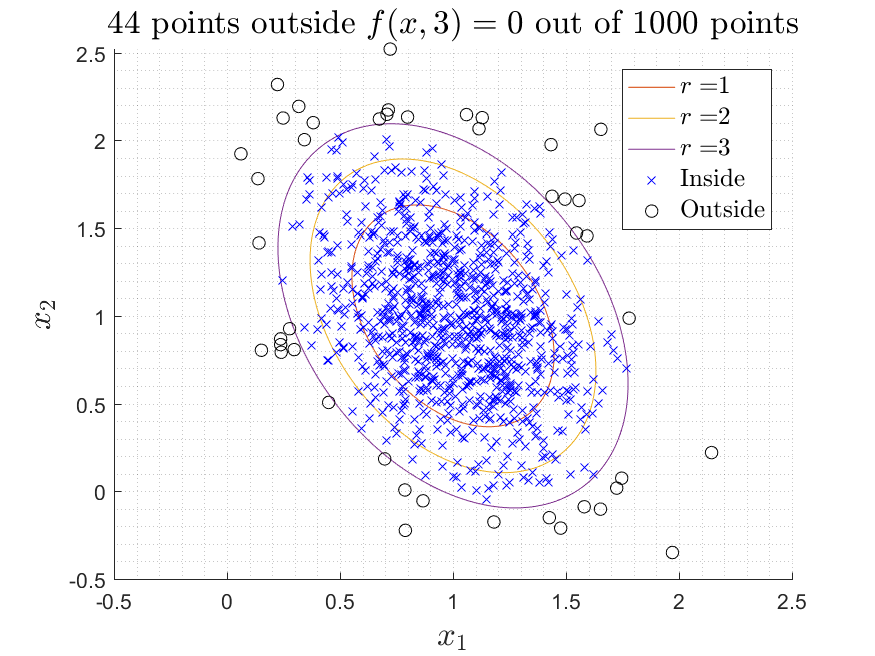
\includegraphics[width=0.65\textwidth]{Figures/plot2_1.png}
	\caption{\label{fig:levelSet} Level set for the function given in Eq. \eqref{eq:multivarFunc}, together with randomly placed points following a 2D multivariate normal distribution.}
\end{figure}

\subsection{Problem} % Problem 2.2

The correlation and covariance matrices for $X$ are computed using the functions \verb|cov()| and \verb|corr()|. To scale each feature between 0 and 1 to make $Y$ each value is divided by the highest number in the data set. The correlation and covariance matrices for both $X$ and $Y$ are plotted and shown in Figures~\ref{fig:cov}. and~\ref{fig:corr}.

\begin{figure}[H]
    \centering
    \begin{subfigure}[b]{0.40\textwidth}
        \centering
        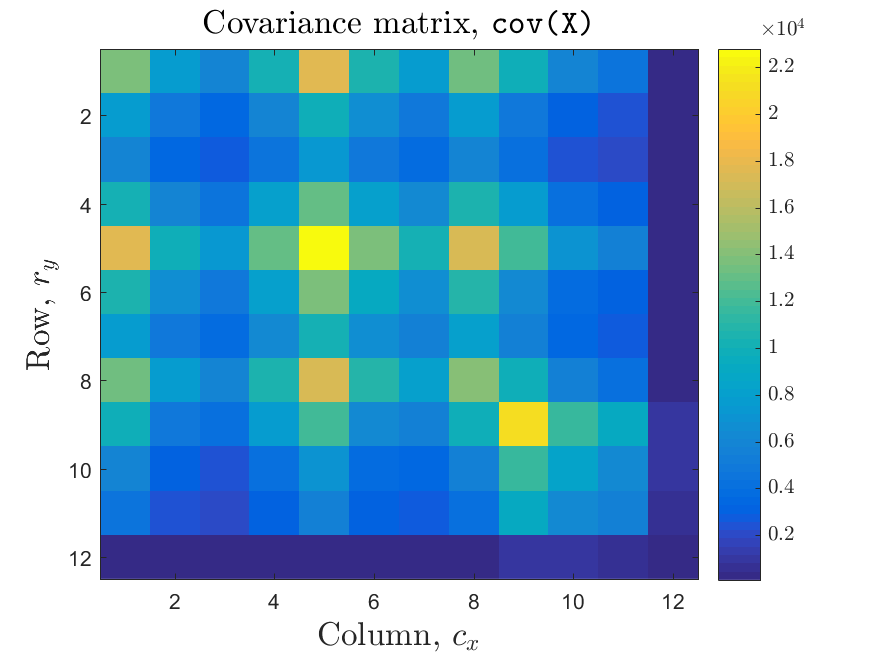
\includegraphics[width=\textwidth]{Figures/plot2_2_cov_x.png}
    \end{subfigure}
    \begin{subfigure}[b]{0.40\textwidth}
        \centering
        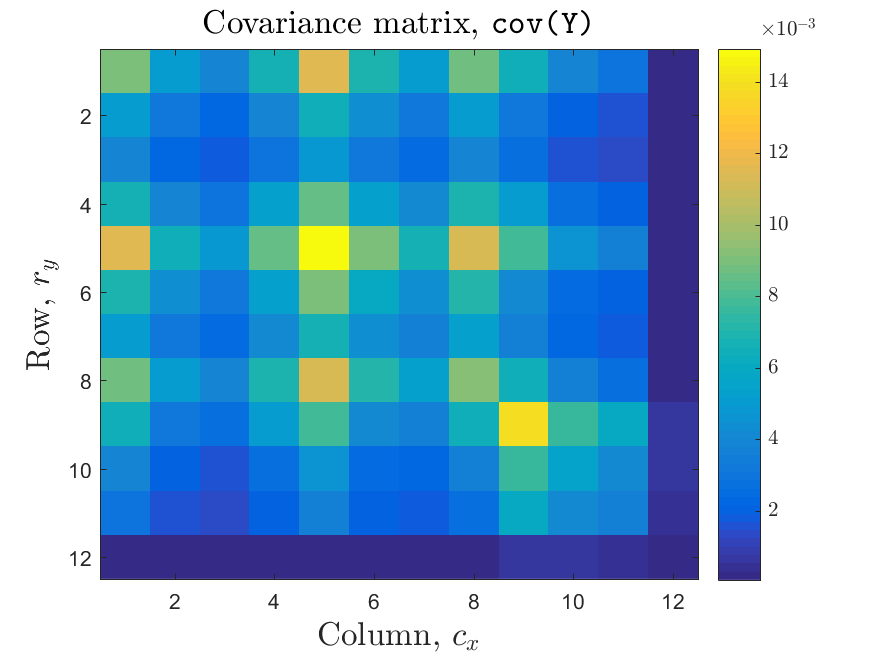
\includegraphics[width=\textwidth]{Figures/plot2_2_cov_y.png}
    \end{subfigure}
    \caption{\label{fig:cov} The covariance of two random variables shows their joint variability. If great values in one variable corresponds to great values in the other and the same is true for small values then the covariance tend to be large. The covariance also contains information of the variance of the variables, therefore there is no surprise that the downscaled matrix $Y$ contains much smaller elements.}
\end{figure}

\begin{figure}[H]
    \centering
    \begin{subfigure}[b]{0.40\textwidth}
        \centering
        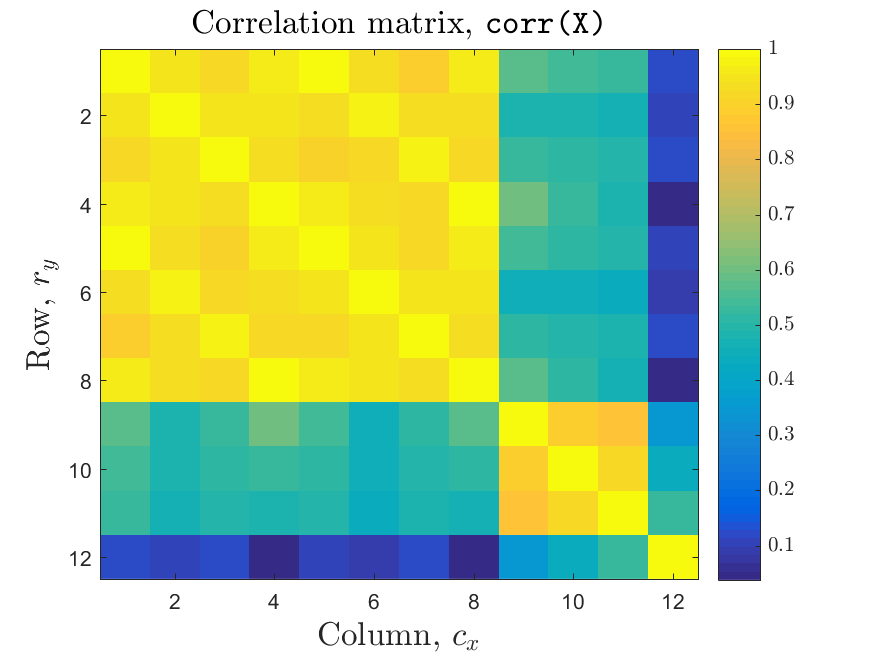
\includegraphics[width=\textwidth]{Figures/plot2_2_corr_x.png}
    \end{subfigure}
    \begin{subfigure}[b]{0.40\textwidth}
        \centering
        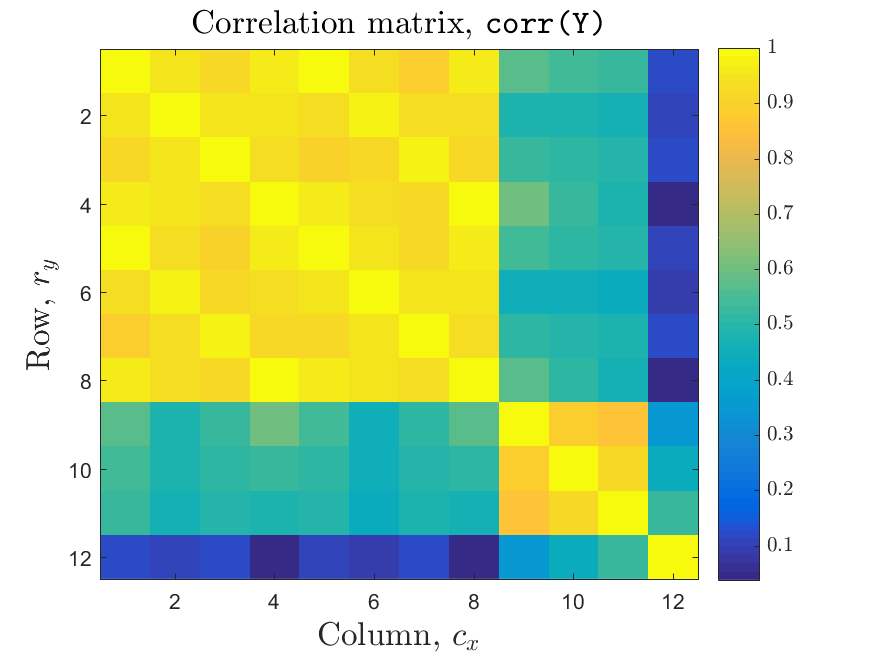
\includegraphics[width=\textwidth]{Figures/plot2_2_corr_y.png}
    \end{subfigure}
    \caption{\label{fig:corr} The correlation of two variables is a measure of how much they correlate, ranging from $1$, positive correlated, to $-1$ negative correlation. It is no surprise that the original matrix $X$ has the same correlation matrix as the normalized matrix $Y$ since all the numbers are scaled in the same manner. }
\end{figure}

\noindent Both the covariance and correlation look identical for both $X$ and $Y$ when visualized. The correlation matrices are identical whereas the covariance matrices don't have the same numerical values but the ratio between values is the same. This was to be expected since $Y$ is just a scaled version of $X$.\\
Lastly the pair with the minimum correlation are plotted. The pair is column 8 and 12. As seen in Figure~\ref{fig:scatter} there are two clear clusters, one where the data points are very close together and the other where the data points are sparsely distributed.

\begin{figure}[H]
    \centering
    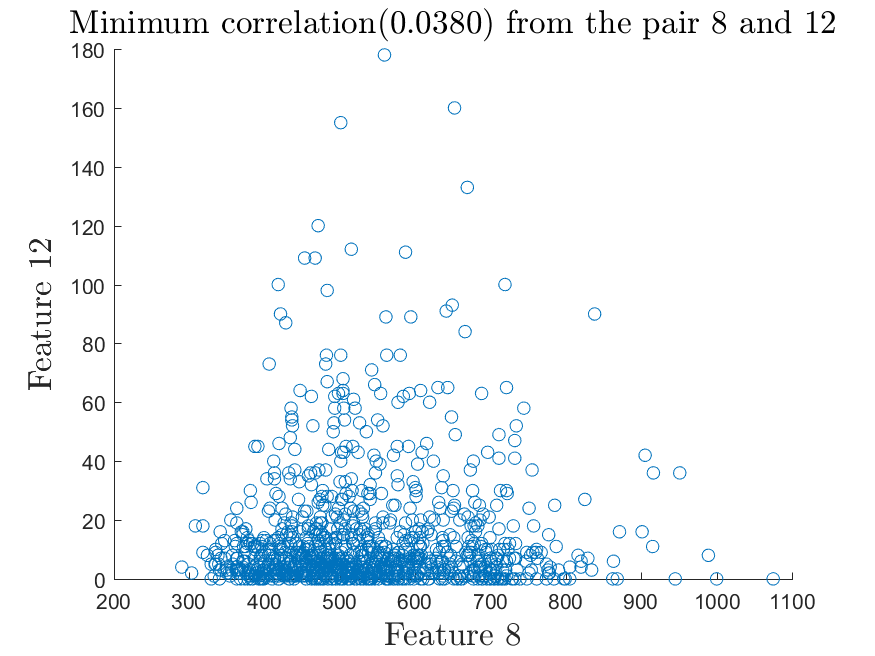
\includegraphics[width=0.4\textwidth]{Figures/plot2_2_scatter.png}
    \caption{The pair of features with minimum correlation are $(8,12)$ and the scattered data from these features. }
    \label{fig:scatter}
\end{figure}



\end{document}
